
\section{Closure Test of Templates in MC}
\label{sec:mc}

The above procedure is applied to MC to test its effectiveness under `ideal' conditions. Templates are derived from PhotonJet MC, 
and these templates are used to predict the MET distribution in ZJets MC. The MC samples used are:
\begin{itemize}
\item PhotonJet MC
  \begin{itemize}
  \item \verb=/G_Pt_15to30_TuneZ2_7TeV_pythia6/Spring11-PU_S1_START311_V1G1-v1/AODSIM  =
  \item \verb=/G_Pt_30to50_TuneZ2_7TeV_pythia6/Spring11-PU_S1_START311_V1G1-v1/AODSIM  =
  \item \verb=/G_Pt_50to80_TuneZ2_7TeV_pythia6/Spring11-PU_S1_START311_V1G1-v1/AODSIM  =
  \item \verb=/G_Pt_80to120_TuneZ2_7TeV_pythia6/Spring11-PU_S1_START311_V1G1-v1/AODSIM =
  \item \verb=/G_Pt_120to170_TuneZ2_7TeV_pythia6/Spring11-PU_S1_START311_V1G1-v1/AODSIM=
  \item \verb=/G_Pt_170to300_TuneZ2_7TeV_pythia6/Spring11-PU_S1_START311_V1G1-v1/AODSIM= 	  
  \end{itemize}
\item ZJet MC
  \begin{itemize}
%or use pythia???
  \item \verb=/DYJetsToLL_TuneD6T_M-50_7TeV-madgraph-tauola/Spring11-PU_S1_START311_V1G1-v1/AODSIM=
  \end{itemize}
\end{itemize}

Good agreement between the observed and predicted MET distributions is observed, as shown in Fig.~\ref{fig:mcclosure}.

\begin{figure}[hbt]
  \begin{center}
    \resizebox{0.8\linewidth}{!}{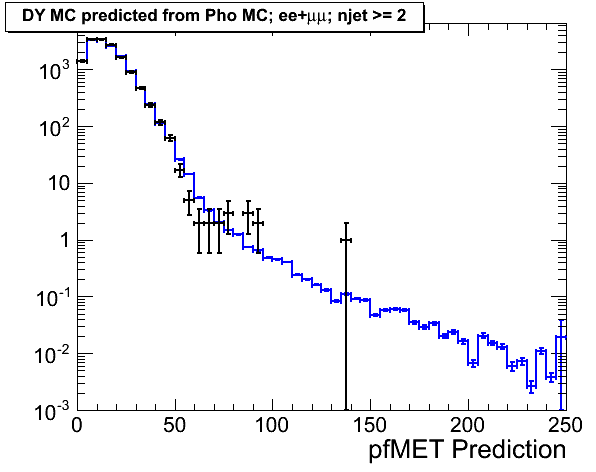
\includegraphics{plots/mcclosure.png}}
	\\ \medskip
    %\resizebox{\linewidth}{!}{
    \begin{tabular}{r|r|r|r}
      MET                   & $>$ 30 GeV & $>$ 60 GeV  & $>$ 120 GeV \\ \hline
      Z+jets observed         &      184   &    10       & 0          \\
      $\gamma$+jets predicted &   182.21   &    11.52    & 1.40       \\
    \end{tabular}
	%}
	\\ \medskip
    %\resizebox{0.5\linewidth}{!}{\includegraphics{plots/MET_pred_3ge_eb_ratio.png}}
    \caption{The MET distribution in Z+jets MC (black) and prediction (blue) for Njet $\ge$ 2. Below the plot is tabulated the integral of the observed Z+jets MC MET and the predicted MET from $\gamma$+jets MC for MET $>$ 30 GeV, $>$ 60 GeV and $>$ 120 GeV. The quantity (observed-predicted)/predicted as a function of MET is shown above the plot.}
    \label{fig:mcclosure}
  \end{center}
\end{figure}


%\begin{wrapfigure}{r}{0.6\textwidth}
%\vspace{-25pt}
%\begin{center}
%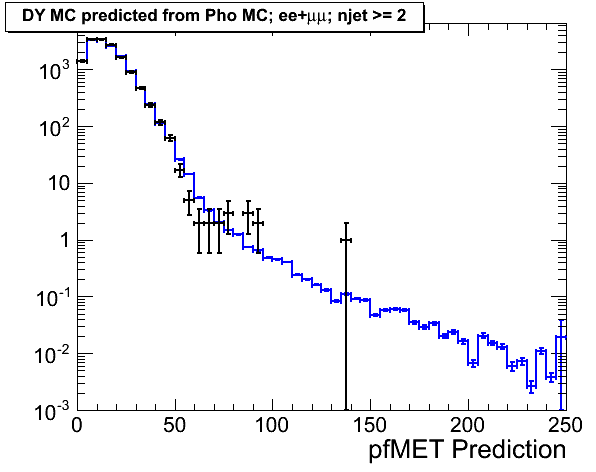
\includegraphics[width=0.8\textwidth]{plots/mcclosure}
% \caption{\label{fig:mcclosure} The MET distribution in Z+jets MC (black) and prediction (blue) for Njet $\ge$ 2. Below the plot is tabulated the integral of the observed Z+jets MC MET and the predicted MET from $\gamma$+jets MC for MET $>$ 30 GeV, $>$ 60 GeV and $>$ 120 GeV. The quantity (observed-predicted)/predicted as a function of MET is shown above the plot.}
%\end{center}
%\vspace{-20pt}
%\end{wrapfigure}
